\documentclass[UTF8,a4paper,11pt]{ctexart}
\usepackage{geometry,booktabs,longtable,float,graphicx,amsmath,amssymb,bm,siunitx}
\usepackage{xcolor,fancyhdr,caption,array,multirow}
\geometry{left=2.15cm,right=2.15cm,top=2.15cm,bottom=2.05cm}
\definecolor{apmblue}{RGB}{31,78,121}
\ctexset{section={format={\Large\bfseries\color{apmblue}}},
subsection={format={\large\bfseries\color{apmblue}}}}
\pagestyle{fancy}\fancyhf{}
\setlength{\headheight}{14pt}
\fancyhead[L]{APMCM B题\quad 问题3多目标优化}
\fancyhead[R]{高性能芯片热管理系统}
\fancyfoot[C]{\thepage}\renewcommand{\headrulewidth}{0.4pt}
\captionsetup{font=small,labelsep=colon}
\setlength{\parindent}{2em}\setlength{\parskip}{2pt}
\setcounter{section}{14}
\title{\textcolor{apmblue}{B题问题3：芯片热管理结构的多目标优化}}
\author{}\date{}

\begin{document}
\maketitle

\section{问题分析与多目标模型}
\subsection{前两问接口与方法取舍}
问题1表明，无量纲热阻$R$衡量整体散热能力，无量纲压降$P$对应水力阻力与泵功代价，无量纲温度非均匀性$U$反映热点风险。三个目标之间存在冲突，不存在同时使三项性能均达到各自最小值的单一方案，因此需先求取Pareto非支配解集，再引入透明的折中准则。

问题2比较了二次OLS、三次OLS、三次Ridge和Mat\'ern高斯过程。三次OLS与Ridge的折外精度几乎相同，均优于二次OLS和高斯过程；考虑高阶项稳定性和统一调用接口，最终三个响应均选用三次Ridge。其OOF-NRMSE分别为$6.555\times10^{-6}$、$0.004626$和$0.004333$。因此本问不再把四类代理模型都当作优化目标函数重复求解，而以问题2已经选定的Ridge为正式目标，以OLS和GP仅作最终点模型分歧审计。这一取舍避免了模型选择与优化算法选择的概念混淆。

有针肋响应统一写为
\[
 \widehat y_k(a,b,N)=\beta_{0k}+\sum_{q=1}^{19}\beta_{qk}
 \frac{\phi_q(\bm\xi)-m_q}{t_q},\qquad k\in\{R,P,U\},
\]
无针肋$(a,N)=(0,0)$使用独立PCHIP支路，不在两类结构之间插值。

\subsection{分段混合设计域}
总可行域为两个不连通集合的并：
\[
\begin{split}
\mathcal D_{\rm pin}&=\{(a,b,N):0.10\le a\le0.30,\ 3\le b\le4.5,\ N\in\{2,4,6,8,10\}\},\\
\mathcal D_0&=\{(0,b,0):3\le b\le4.5\},\qquad \mathcal D=\mathcal D_{\rm pin}\cup\mathcal D_0.
\end{split}
\]
$N$始终枚举，不连续化；$a=0,N>0$与$a>0,N=0$均为非法结构。优化模型为
\[
 \min_{\bm x\in\mathcal D}\bm F(\bm x)
 =\min_{\bm x\in\mathcal D}\bigl(\widehat R(\bm x),\widehat P(\bm x),\widehat U(\bm x)\bigr).
\]
题目没有给出性能硬阈值，故不虚构额外约束，代理模型的合法插值域即为本问边界。

\subsection{锚点、收益矩阵与统一尺度}
分别最小化$R,P,U$得到三个单目标锚点$\bm x_R^*,\bm x_P^*,\bm x_U^*$，其全目标响应构成收益矩阵。理想点取各列单目标最小值，初始Nadir点取收益矩阵各行最大值；合并参考前沿后再作覆盖检查。本次覆盖检查把最终统一标尺确定为
\[
 \bm F^{\rm I}=(0.720227,\ 0.076040,\ 0.771787),\qquad
 \bm F^{\rm N}=(0.760176,\ 0.158555,\ 0.819442).
\]
定义$z_k=(F_k-F_k^{\rm I})/(F_k^{\rm N}-F_k^{\rm I})$。Pareto筛选仍使用原始响应；归一化只用于算法指标与折中决策。

\section{候选优化算法与比较准则}
\subsection{候选一：分层致密网格}
对每个合法$N$分别建立$101\times101$、$201\times201$和$401\times401$的$(a,b)$网格；无针肋支路在$b\in[3,4.5]$上取2001点。各层先筛选非支配点，再作全局合并。由于代理模型为显式三次多项式，网格可确定性覆盖完整低维设计域，适合作为主参考。

\subsection{候选二：按$N$分层的NSGA-II}
为避免遗传算子产生非法排数，对五个$N$水平分别运行二维NSGA-II，再合并各层非支配解。使用模拟二进制交叉和多项式变异，交叉概率0.90、分布指数15，单变量变异概率$1/2$、分布指数20。候选比较采用种群60、50代和20个独立种子；每次分层运行共评价15300次。此设置的目的在于以较低代价独立验证前沿位置和最终折中点，而非替代确定性致密网格。

\subsection{局部连续精化}
致密网格仍受步长限制。固定问题2锚点确定的$\bm F^{\rm I},\bm F^{\rm N}$，对每个合法$N$直接求解
\[
 \min_{0.1\le a\le0.3,\ 3\le b\le4.5}C_{\rm AT}(a,b,N).
\]
以401网格折中点和NSGA-II点作为初值，先用差分进化定位，再以多起点SLSQP精修；无针肋分支用一维有界连续优化。五个有针肋层最优和无针肋最优组成$\mathcal P_{\rm local}$，既用于比较各层评分，也进入统一参考集。

\subsection{未选方法的定位}
单一加权和可能遗漏非凸前沿，也不能展示完整权衡，故不作为主搜索器；TOPSIS是Pareto集后的决策方法，不能替代连续域搜索；增强切比雪夫用于最终折中选择，而不是人为包装成第三套前沿算法。这样的候选集合与本题两个连续变量、一个低基数离散变量的结构相匹配。

\subsection{统一比较指标}
所有方法使用相同$\bm F^{\rm I},\bm F^{\rm N}$。为消除以401网格评价自身造成的循环偏向，统一参考集定义为
\[
 \mathcal P_{\rm ref}=\operatorname{ND}\!\left(
 \mathcal P_{401}\cup\bigcup_{r=1}^{20}\mathcal P_{{\rm NSGA},r}
 \cup\mathcal P_{\rm local}\right),
\]
本次合并后含18183个非支配点。所有方法均相对于该集合计算IGD+。HV参考点固定为$\bm r=(1.10,1.10,1.10)$，采用沿第一目标扫描、对二维截面矩形并集精确积分的三维算法：
\[
HV(\mathcal P;\bm r)=\operatorname{Vol}\!\left(
\bigcup_{\bm z\in\mathcal P}[z_R,r_R]\times[z_P,r_P]\times[z_U,r_U]\right).
\]
Spacing为归一化前沿最近邻距离的标准差。HV越大越好，IGD+与Spacing越小越好。

\section{算法比较与Pareto结果}
\subsection{网格收敛与随机算法复核}
表\ref{tab:algorithm}表明，网格由101加密至401时精确HV单调增加，IGD+与Spacing持续下降；201与401网格给出的综合折中点均约为$(0.225,4.5,6)$，位置不再变化。精确HV满足
\[
\frac{HV_{401}-HV_{201}}{HV_{201}}=4.21\times10^{-4}<10^{-3},
\]
故网格达到预设收敛精度。20次NSGA-II的平均HV为$0.892203\pm0.001348$；其IGD+为$0.011923\pm0.002173$，说明受较小评价预算影响，随机前沿覆盖较疏。401网格相对合并参考集的IGD+为$1.40\times10^{-5}$而非人为置零，因而比较不再循环定义。最终以401网格作为确定性主参考，以NSGA-II和局部精化作为独立复核。

\begin{table}[H]\centering\small
\caption{候选优化算法的统一指标比较}\label{tab:algorithm}
\begin{tabular}{lrrrrrr}
\toprule
方法 & 非支配点 & HV & IGD+ & Spacing & 时间/s & 评价次数\\
\midrule
101网格 & 1362 & 0.902914 & 0.001239 & 0.002824 & 0.96 & 53006\\
201网格 & 4679 & 0.903767 & 0.000503 & 0.001314 & 2.94 & 204006\\
401网格 & 16858 & 0.904148 & 0.000014 & 0.000624 & 10.13 & 806006\\
NSGA-II（20次均值） & 107.95 & 0.892203 & 0.011923 & 0.017331 & 0.94 & 15300\\
NSGA-II（标准差） & 3.05 & 0.001348 & 0.002173 & 0.002833 & 0.08 & 0\\
\bottomrule
\end{tabular}
\end{table}

\begin{figure}[H]\centering
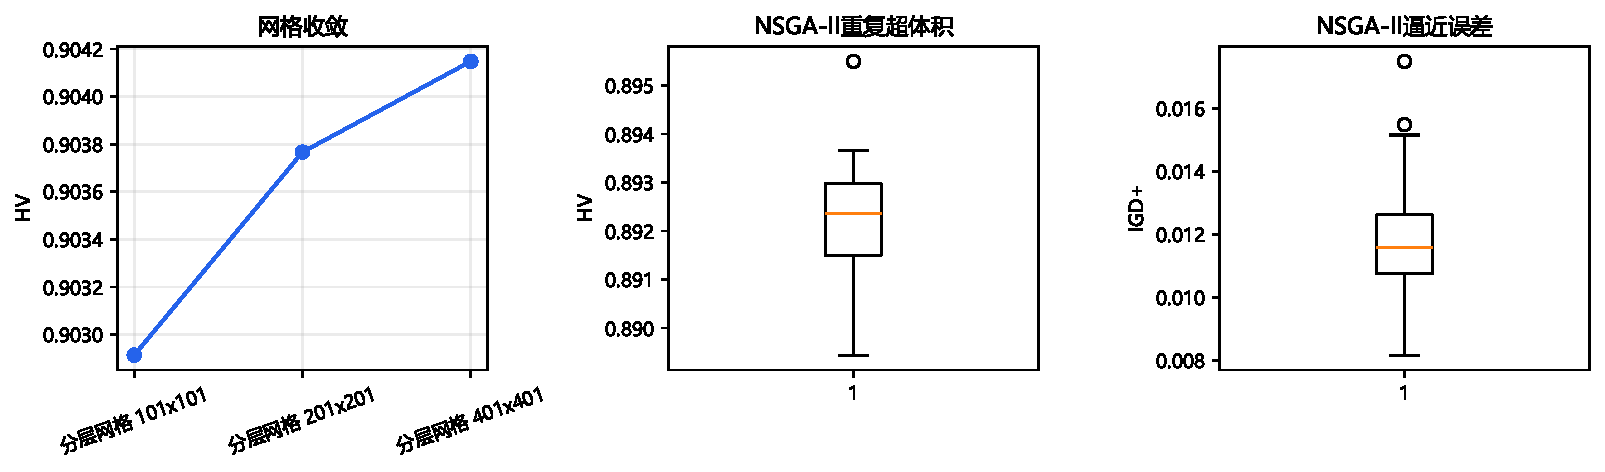
\includegraphics[width=.94\linewidth]{../../05_figures/q3/fig_q3_04_algorithm_comparison.pdf}
\caption{精确HV的三级网格收敛与20次NSGA-II重复比较；IGD+统一相对于合并参考集计算。虚线为401网格值。}\label{fig:algorithm}
\end{figure}

\subsection{全局Pareto前沿}
401网格共评价806006个合法方案，得到16858个全局非支配点。2001个无针肋候选在分支内部均非支配，但与有针肋方案全局合并后保留0个，说明在本数据覆盖域内，无针肋结构的低压降优势不足以同时补偿其热阻与温度非均匀性损失。该结论来自全局比较，并非预先删除无针肋分支。

图\ref{fig:pareto}显示前沿由多个离散$N$层共同构成。小$N$有利于降低压降；较大$N$可降低热阻但增加水力代价，且温度均匀性在中等排数附近更优。NSGA-II合并结果找到的最佳折中点为$(0.224642,4.5,6)$，评分0.386390；连续精化结果为$(0.224932,4.5,6)$，评分0.386383。三者高度一致，从而验证最终结构位置不依赖单一算法。

\begin{figure}[H]\centering
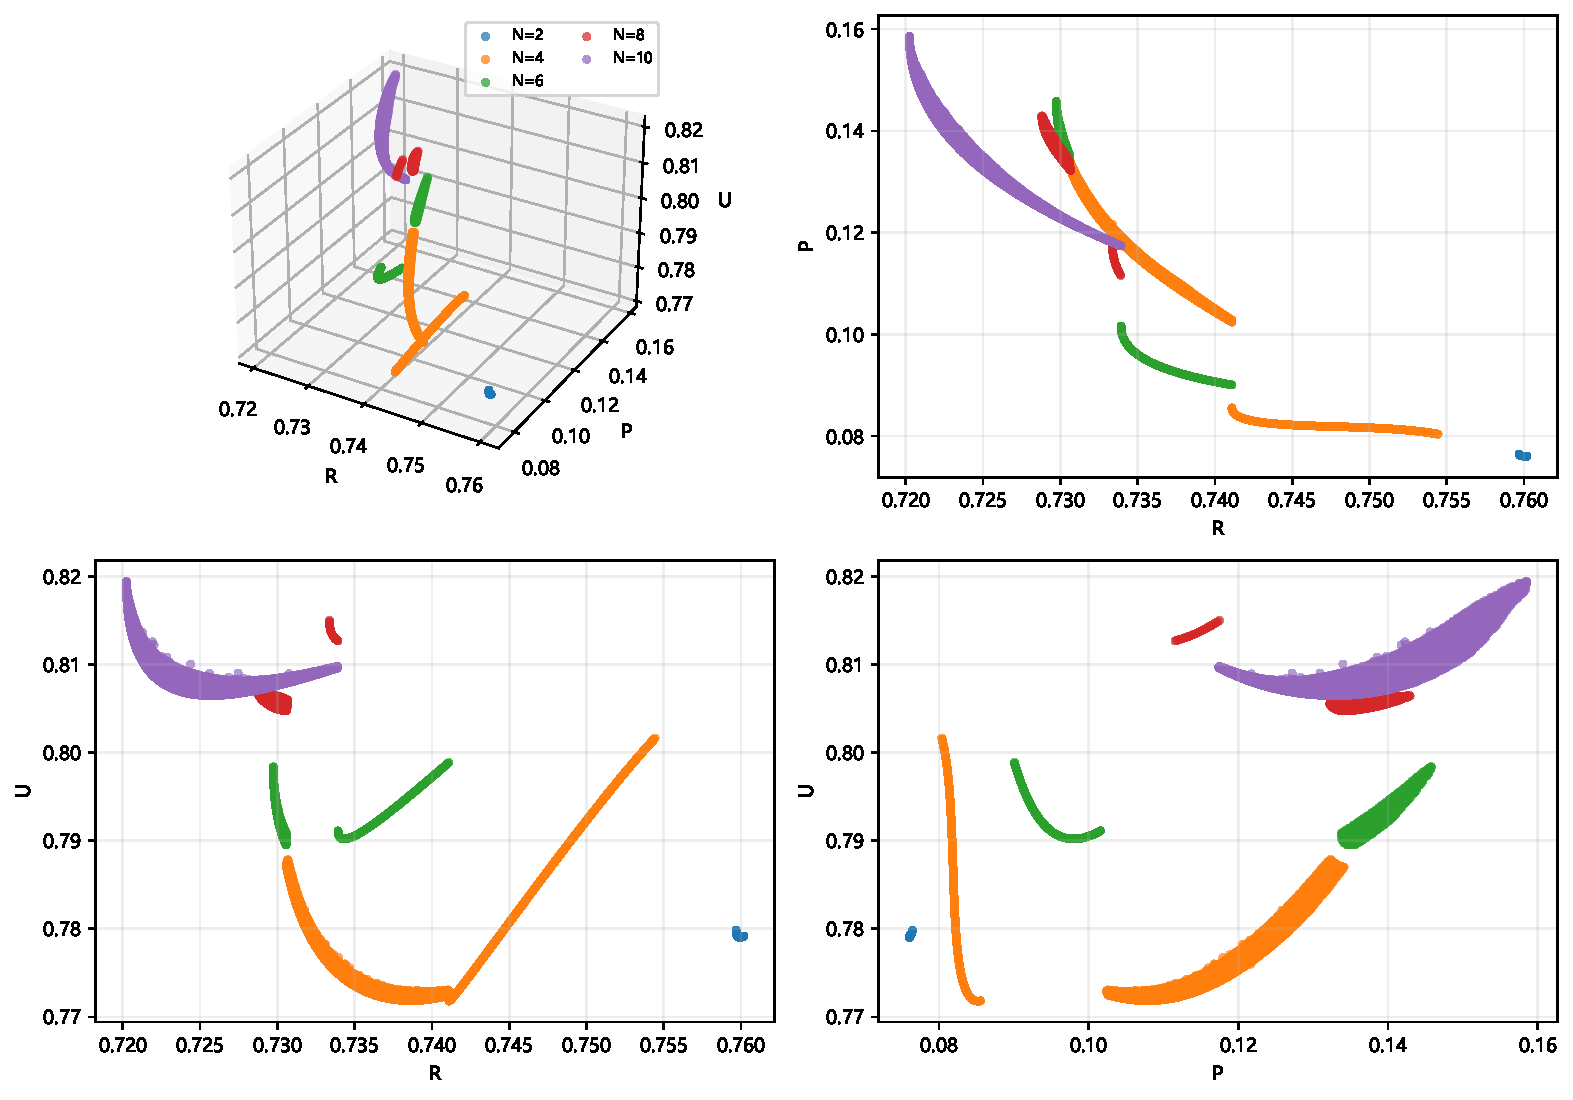
\includegraphics[width=.95\linewidth]{../../05_figures/q3/fig_q3_01_pareto_front.pdf}
\caption{合并参考Pareto前沿及两两投影，四个子图均使用原始无量纲响应。颜色区分排数$N$；星号标出三个单目标锚点和连续精化综合方案，灰色叉号表示被支配的无针肋基线。}\label{fig:pareto}
\end{figure}

\section{综合最优方案与可信度审计}
\subsection{等权增强切比雪夫折中}
问题4将进一步讨论权重变化，因此本问采用无额外偏好的等尺度平衡准则：
\[
 C_{\rm AT}(\bm x)=\max\{z_R,z_P,z_U\}
 +10^{-4}(z_R+z_P+z_U),\qquad
 \bm x^*=\arg\min_{\bm x\in\mathcal P_{\rm ref}}C_{\rm AT}(\bm x).
\]
主项最小化三项指标中最差的标准化退让，小的增强项只用于打破并列。另以
\[
C_2=\sqrt{(z_R^2+z_P^2+z_U^2)/3}
\]
寻找最近理想点，作为范数敏感性校验。

\begin{table}[H]\centering\small
\caption{单目标锚点、连续精化方案与工程基准比较}\label{tab:candidates}
\begin{tabular}{lrrrrrrrr}
\toprule
方案 & $a$ & $b$ & $N$ & $R$ & $P$ & $U$ & $C_{\rm AT}$ & 状态\\
\midrule
最小热阻锚点 & .2320 & 3.0675 & 10 & .720227 & .158525 & .819424 & .9998 & Pareto\\
最小压降锚点 & .2285 & 4.5000 & 2 & .760176 & .076040 & .779150 & 1.0001 & Pareto\\
最小非均匀性锚点 & .2250 & 4.5000 & 4 & .741104 & .085238 & .771787 & .5226 & Pareto\\
连续精化综合最优 & .2249 & 4.5000 & 6 & .734330 & .097996 & .790195 & .3864 & Pareto\\
NSGA-II验证点 & .2246 & 4.5000 & 6 & .734345 & .097933 & .790195 & .3864 & Pareto\\
最近理想点 & .2240 & 4.5000 & 4 & .741114 & .085126 & .771790 & .5229 & Pareto\\
最佳原始样本 & .2000 & 4.5000 & 6 & .736613 & .093468 & .792252 & .4295 & 样本基准\\
无针肋最佳折中 & 0 & 4.0000 & 0 & .767907 & .088704 & .838398 & 1.3980 & 被支配\\
\bottomrule
\end{tabular}
\end{table}

最终推荐
\[
 \boxed{a^*=0.224932,\qquad b^*=4.500000,\qquad N^*=6},
\]
其预测性能为$(R,P,U)=(0.734330,0.097996,0.790195)$。相对最佳原始样本，增强切比雪夫综合评分由0.4295降至0.3864，降低约$10.05\%$；该比例不代表三项物理性能均提高$10.05\%$。最近同层样本为$(0.20,4.5,6)$，标准化设计距离约0.125。最近理想点偏向$N=4$的低$U$方案，说明$L_2$更强调总体距离，而增强切比雪夫更严格控制最大退让；两种准则的差异来自可解释的范数偏好。无针肋最佳折中位于$b\approx4.0$，且被$(a,b,N)=(0.2276,4.5,4)$等有针肋方案同时改善三项目标，说明针肋带来的热阻和均匀性收益足以抵消其压降代价。

\begin{figure}[H]\centering
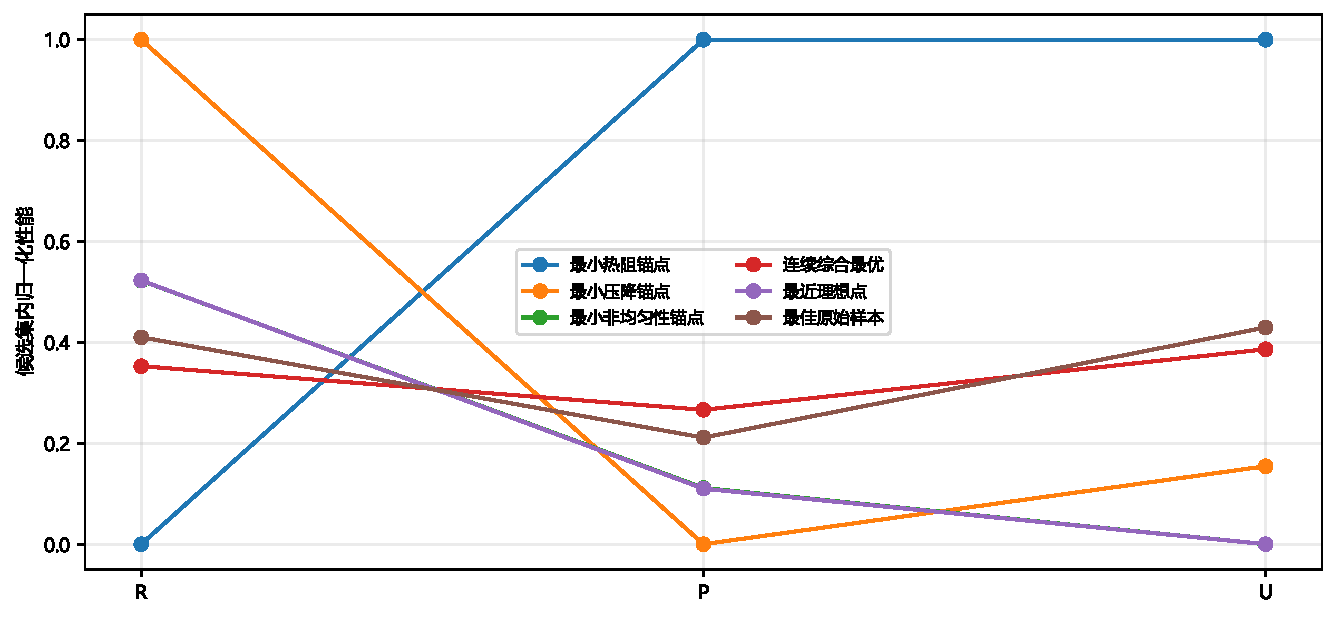
\includegraphics[width=.88\linewidth]{../../05_figures/q3/fig_q3_02_candidate_comparison.pdf}
\caption{候选方案在统一归一化尺度下的平行坐标比较。}\label{fig:parallel}
\end{figure}

\subsection{代理模型与邻域稳定性}
在最终点调用问题2保留的三次OLS和Mat\'ern GP作审计，结果见表\ref{tab:audit}。三类模型的最大分歧占有效目标范围的比例分别约为$0.38\%$、$0.34\%$和$1.10\%$，没有改变综合结论。基于问题2折外MaxAE，Ridge预测的经验误差带为
\[
R=0.734330\pm7.631\times10^{-7},\quad
P=0.097996\pm0.004200,\quad
U=0.790195\pm0.001817.
\]
这些只是折外最大误差尺度，不是统计置信区间。

\begin{table}[H]\centering\small
\caption{最终方案的代理模型审计}\label{tab:audit}
\begin{tabular}{lrrr}
\toprule 模型 & $R$ & $P$ & $U$\\\midrule
三次Ridge（正式目标） & 0.734330 & 0.097996 & 0.790195\\
三次OLS & 0.734330 & 0.097997 & 0.790190\\
Mat\'ern GP & 0.734483 & 0.098277 & 0.790716\\
归一化最大分歧 & 0.0038 & 0.0034 & 0.0110\\
\bottomrule
\end{tabular}
\end{table}

将$a$在最优值附近分别减、加0.005时，$C_{\rm AT}$为0.3884和0.3885；将$b$从4.50内移至4.48时评分为0.3965，变化平缓。相邻排数$N=4,8$的评分分别为0.5227和0.8517，表明排数选择比小幅连续参数扰动更敏感。最终点位于$b=4.5$的合法边界，只能说明附件覆盖域内边界最优，不能外推$b>4.5$仍会改善。

\begin{figure}[H]\centering
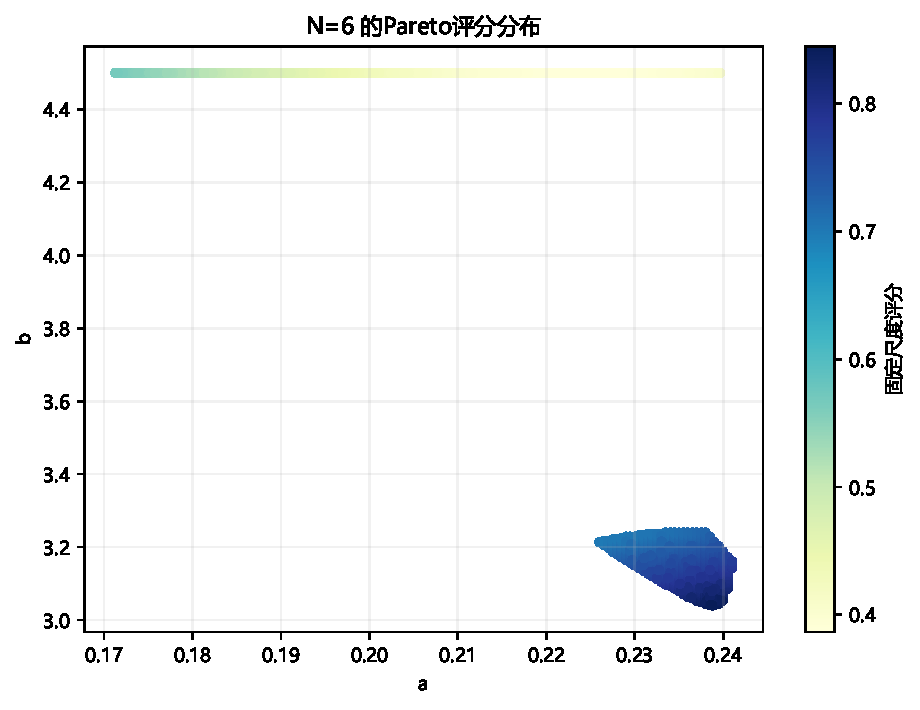
\includegraphics[width=.60\linewidth]{../../05_figures/q3/fig_q3_03_design_slice.pdf}
\caption{$N=6$完整合法矩形域上的综合评分。黑色空心点为该层Pareto点，红色星号为边界上的连续精化最优。}\label{fig:slice}
\end{figure}

\section{问题3结论}
三级网格、20次分层NSGA-II、局部连续精化和独立无针肋支路共同构成多算法闭环。IGD+统一相对于18183点合并参考集计算，HV采用精确三维算法；网格加密的HV相对变化低于$10^{-3}$。401网格覆盖最完整，NSGA-II以约$1.9\%$的评价次数找到同一折中区域，连续精化最终选择$(a,b,N)=(0.224932,4.5,6)$。该方案属于全局非支配集，相对最佳原始样本的增强切比雪夫综合评分降低约$10.05\%$，且OLS、GP审计与局部扰动均未显示代理模型尖峰。权重变化应留给问题4，工况扰动和鲁棒性则留给问题5。

\section*{参考文献}
\noindent[1] DEB K, PRATAP A, AGARWAL S, et al. A fast and elitist multiobjective genetic algorithm: NSGA-II[J]. IEEE Transactions on Evolutionary Computation, 2002, 6(2): 182--197.

\end{document}
